% !TEX root = BA-Bauer.tex

\subsection{Autodesk EAGLE}
Die Schaltpläne und das Design der Platine wird in der \textit{Electronic Design Automation} (EDA) Software \textit{EAGLE} der Firma \textit{Autodesk} entwickelt. Innerhalb der Software können Schaltpläne erstellt werden. Anhand dieser Schaltung kann dann ein entsprechendes Layout der zu fertigenden Platine erstellt werden. Zuletzt können Produktionsdaten exportiert werden, mit denen die Platine industriell hergestellt werden kann \cite{eagle_homepage}.\\
Für die Erstellung des Schaltplans und Platinenlayouts wird eine Bauteilbibliothek benötigt. \textit{EAGLE} beinhaltet bereits initial eine große Bibliothek mit verschiedensten Bauteilen vieler Hersteller, jedoch umfasst diese nicht alle am Markt verfügbaren Bauteile. Viele der in dieser Arbeit verwendeten Bauteile befinden sich nicht darin, weswegen eine eigene Bauteilbibliothek erstellt und explizit für die Entwicklung verwendet wird. Zudem soll dadurch das Fehlerrisiko in Bezug auf die Bauteilabmessungen und Pinbelegung reduziert werden. Ein Bauteil der Bauteilbibliothek besteht aus Sicht der Software aus drei Teilen. Dem $symbol$ (Abbildung \ref{fig:eagle-sym}), dem $footprint$ (Abbildung \ref{fig:eagle-foot}) und einem 3D-Modell (Abbildung \ref{fig:eagle-3d}).
\begin{figure}[h]
	\centering
	\begin{minipage}{.3\linewidth}
		\centering
		\includegraphics[height=.1\textheight]{lib-symbol}
		\caption{EAGLE Symbol}
		\label{fig:eagle-sym}
	\end{minipage}
	\hfill
	\begin{minipage}{.3\linewidth}
		\centering
		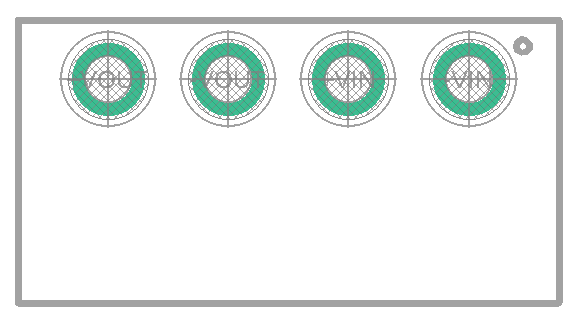
\includegraphics[height=.1\textheight]{lib-footprint}
		\caption{EAGLE Footprint}
		\label{fig:eagle-foot}
	\end{minipage}
	\hfill
	\begin{minipage}{.3\linewidth}
		\centering
		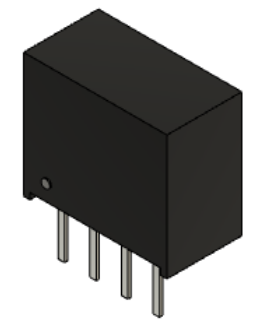
\includegraphics[height=.1\textheight]{lib-3d}
		\caption{EAGLE 3D-Modell}
		\label{fig:eagle-3d}
	\end{minipage}
\end{figure}
Das Symbol wird für die Entwicklung des Schaltplans verwendet und besitzt keine elektrischen Eigenschaften oder Dimensionen. Eine Simulation der Schaltung ist dementsprechend in $EAGLE$ nicht möglich. Die Anschlüsse der Symbole können im Schaltplan mit Leitungen verbunden werden. Um den Schaltplan auf die Hardwareebene zu projizieren, wird ein zugehöriger \textit{footprint} benötigt. Dieser enthält die Dimensionen und Anordnung der entsprechenden Lötstellen des Bauteils, welche in der Regel vom Hersteller des Bauteils zur Verfügung gestellt werden. Im Bibliotheks-Manager in \textit{EAGLE} werden dann die Anschlüsse des Symbols den entsprechenden Lötstellen des \textit{footprints} zugeordnet. Die Verbindung zwischen Schaltplan und Platine ist nun hergestellt. Um  einen noch realistischeren Entwurf der Platine einsehen zu können, kann ein 3D-Modell des Bauteils eingefügt werden. Standard Bauteile wie SMD-Kondensatoren, -Widerstände oder gängige Chip-Gehäuse können mit einem in \textit{EAGLE} integrierten Generator erzeugt werden. Mit den vom Hersteller des Bauteils angegebenen Dimensionen und Toleranzen erzeugt der Generator einen \textit{footprint} mit einem dazugehörigen 3D-Modell des Bauteils. Handelt es sich bei dem Bauteil nicht um ein Standard-Bauteil, so muss der \textit{footprint} in $EAGLE$ und das 3D-Modell in einer externen CAD-Software konstruiert werden. Über den Bibliotheks-Manager kann dann das 3D-Modell bezogen auf den \textit{footprint} dreidimensional platziert werden. Mithilfe der 3D-Modelle kann EAGLE in Verbindung mit der Software \textit{Fusion 360} der Firma \textit{Autodesk} ein 3D-Modell der gesamten Platine inklusive aller Bauteile, für die entsprechende 3D-Modelle in der Bauteilbibliothek existieren, exportieren. Dieses kann dazu verwendet werden, Kollisionen zwischen verschiedenen Bauteilen oder zwischen Bauteilen und Gehäuse vor der Fertigung der Platine zu erkennen oder ein passendes Gehäuse für die Platine zu entwerfen.\\
Mithilfe der in \textit{EAGLE} integrierten sogenannten \textit{Forward-Back-Annotation} werden Änderungen im Schaltplan unmittelbar in das Platinenlayout übertragen. Wird Beispielsweise nur der Wert eines Widerstandes im Schaltplan geändert, so ändert sich auch die Beschriftung des Bauteils auf der Platine. Außerdem werden in der Schaltung gesetzte Verbindungen im Platinenlayout dargestellt. Damit wird das Verlegen von Leiterbahnen vereinfacht und kann fehlerfrei durchgeführt werden. Im Schaltplan nicht bestehende Verbindungen können im Platinenlayout nicht hergestellt werden.
\begin{figure}[h]
	\centering	\begin{minipage}{.35\linewidth}
		\centering
		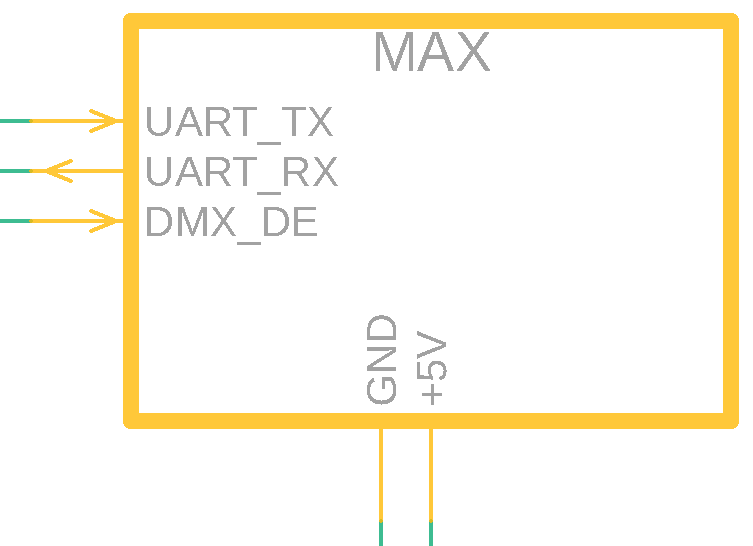
\includegraphics[height=.13\textheight]{Module}
		\caption{Modul $"$MAX$"$}
		\label{fig:module}
	\end{minipage}
	\hfill
	\begin{minipage}{.6\linewidth}
		\centering
		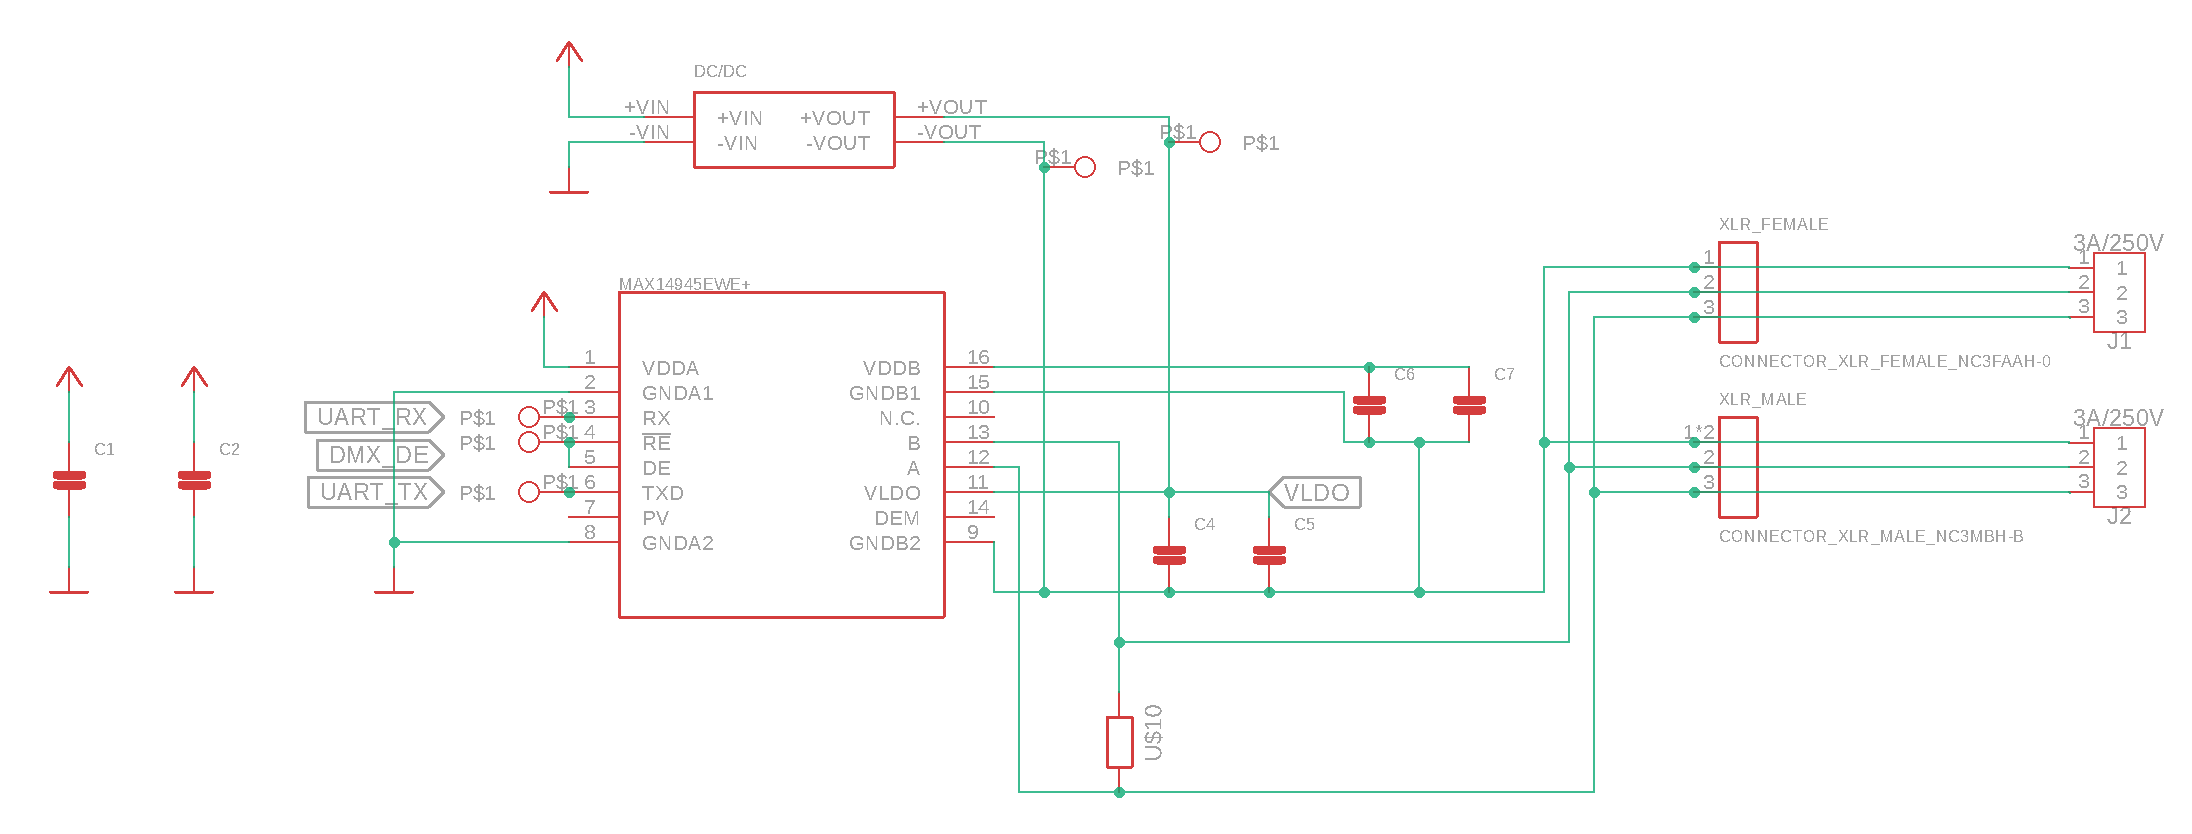
\includegraphics[height=.13\textheight]{Module-schematic}
		\caption{Inhalt des Moduls $"$MAX$"$}
		\label{fig:module-schematic}
	\end{minipage}
\end{figure}
Um die Schaltung möglichst übersichtlich zu gestalten, werden sogenannte \textit{Module} verwendet, durch die komplexe Schaltungen in kleinere \textit{$"$Black-Boxes$"$}\footnote{Box mit Ein-, Ausgängen und unbekanntem Inhalt} heruntergebrochen werden können. Abbildung \ref{fig:module-schematic} und \ref{fig:module} zeigen diese Vereinfachung. Zudem können Module mehrfach in einer Schaltung eingefügt werden. Änderungen in einem Modul wirken sich auf alle eingefügten aus. Verbindungen (grüne Linien in Abbildung \ref{fig:module-schematic}) zwischen Bauteilen werden Namen (\textit{net-names}) zugewiesen, die nur innerhalb des Moduls bekannt sind. Mithilfe der \textit{net-names} können sogenannte \textit{Ports} aus dem Modul herausgeführt werden, womit Verbindungen zu anderen Modulen oder einfachen Bauteilen hergestellt werden können. Pfeile an den $Ports$ signalisieren die Flussrichtung von Signalen, nicht vorhandene Pfeilspitzen signalisieren einen Anschluss einer Spannungsversorgung.\\